\section*{Problem 1} \label{sec:problem1}


% problem introduction
\begin{tcolorbox}[colback=red!5!white,boxrule=0pt,frame empty]
    Use wavelet decomposition (\verb|wavedec|) to decompose an audio signal (\verb|Q1.mat|, sample rate \verb|8192| Hz)
    three level decomposition using \verb|db1|.
\end{tcolorbox}

\vspace{0.5cm}

\begin{figure}[H]
    \centering
    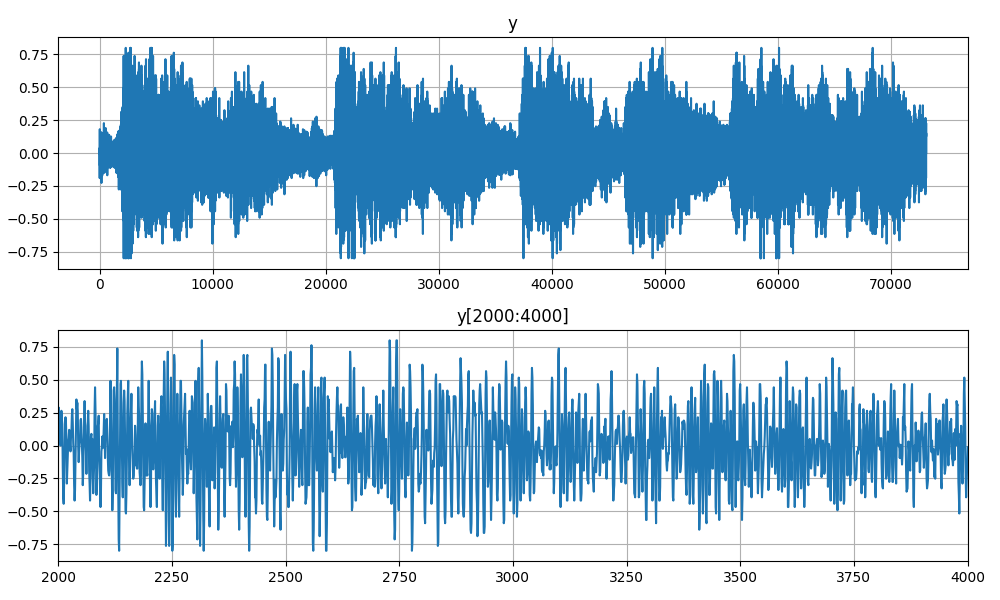
\includegraphics[width=\textwidth]{./img/Q1.png}
    \caption{The audio signal stored in $y$, sample rate 8192 Hz.}
    \label{fig:Q1}
\end{figure}

\vspace{0.5cm}
 

% -- PROBLEM 1.A --------------------------------------------------------------
\begin{tcolorbox}[colback=red!5!white,colframe=red!75!black,title=Problem 1.a]
    Plot the approximated and detailed coefficients.
\end{tcolorbox}


\begin{figure}[H]
    \centering
    % thanks Jens
    \makebox[\textwidth][c]{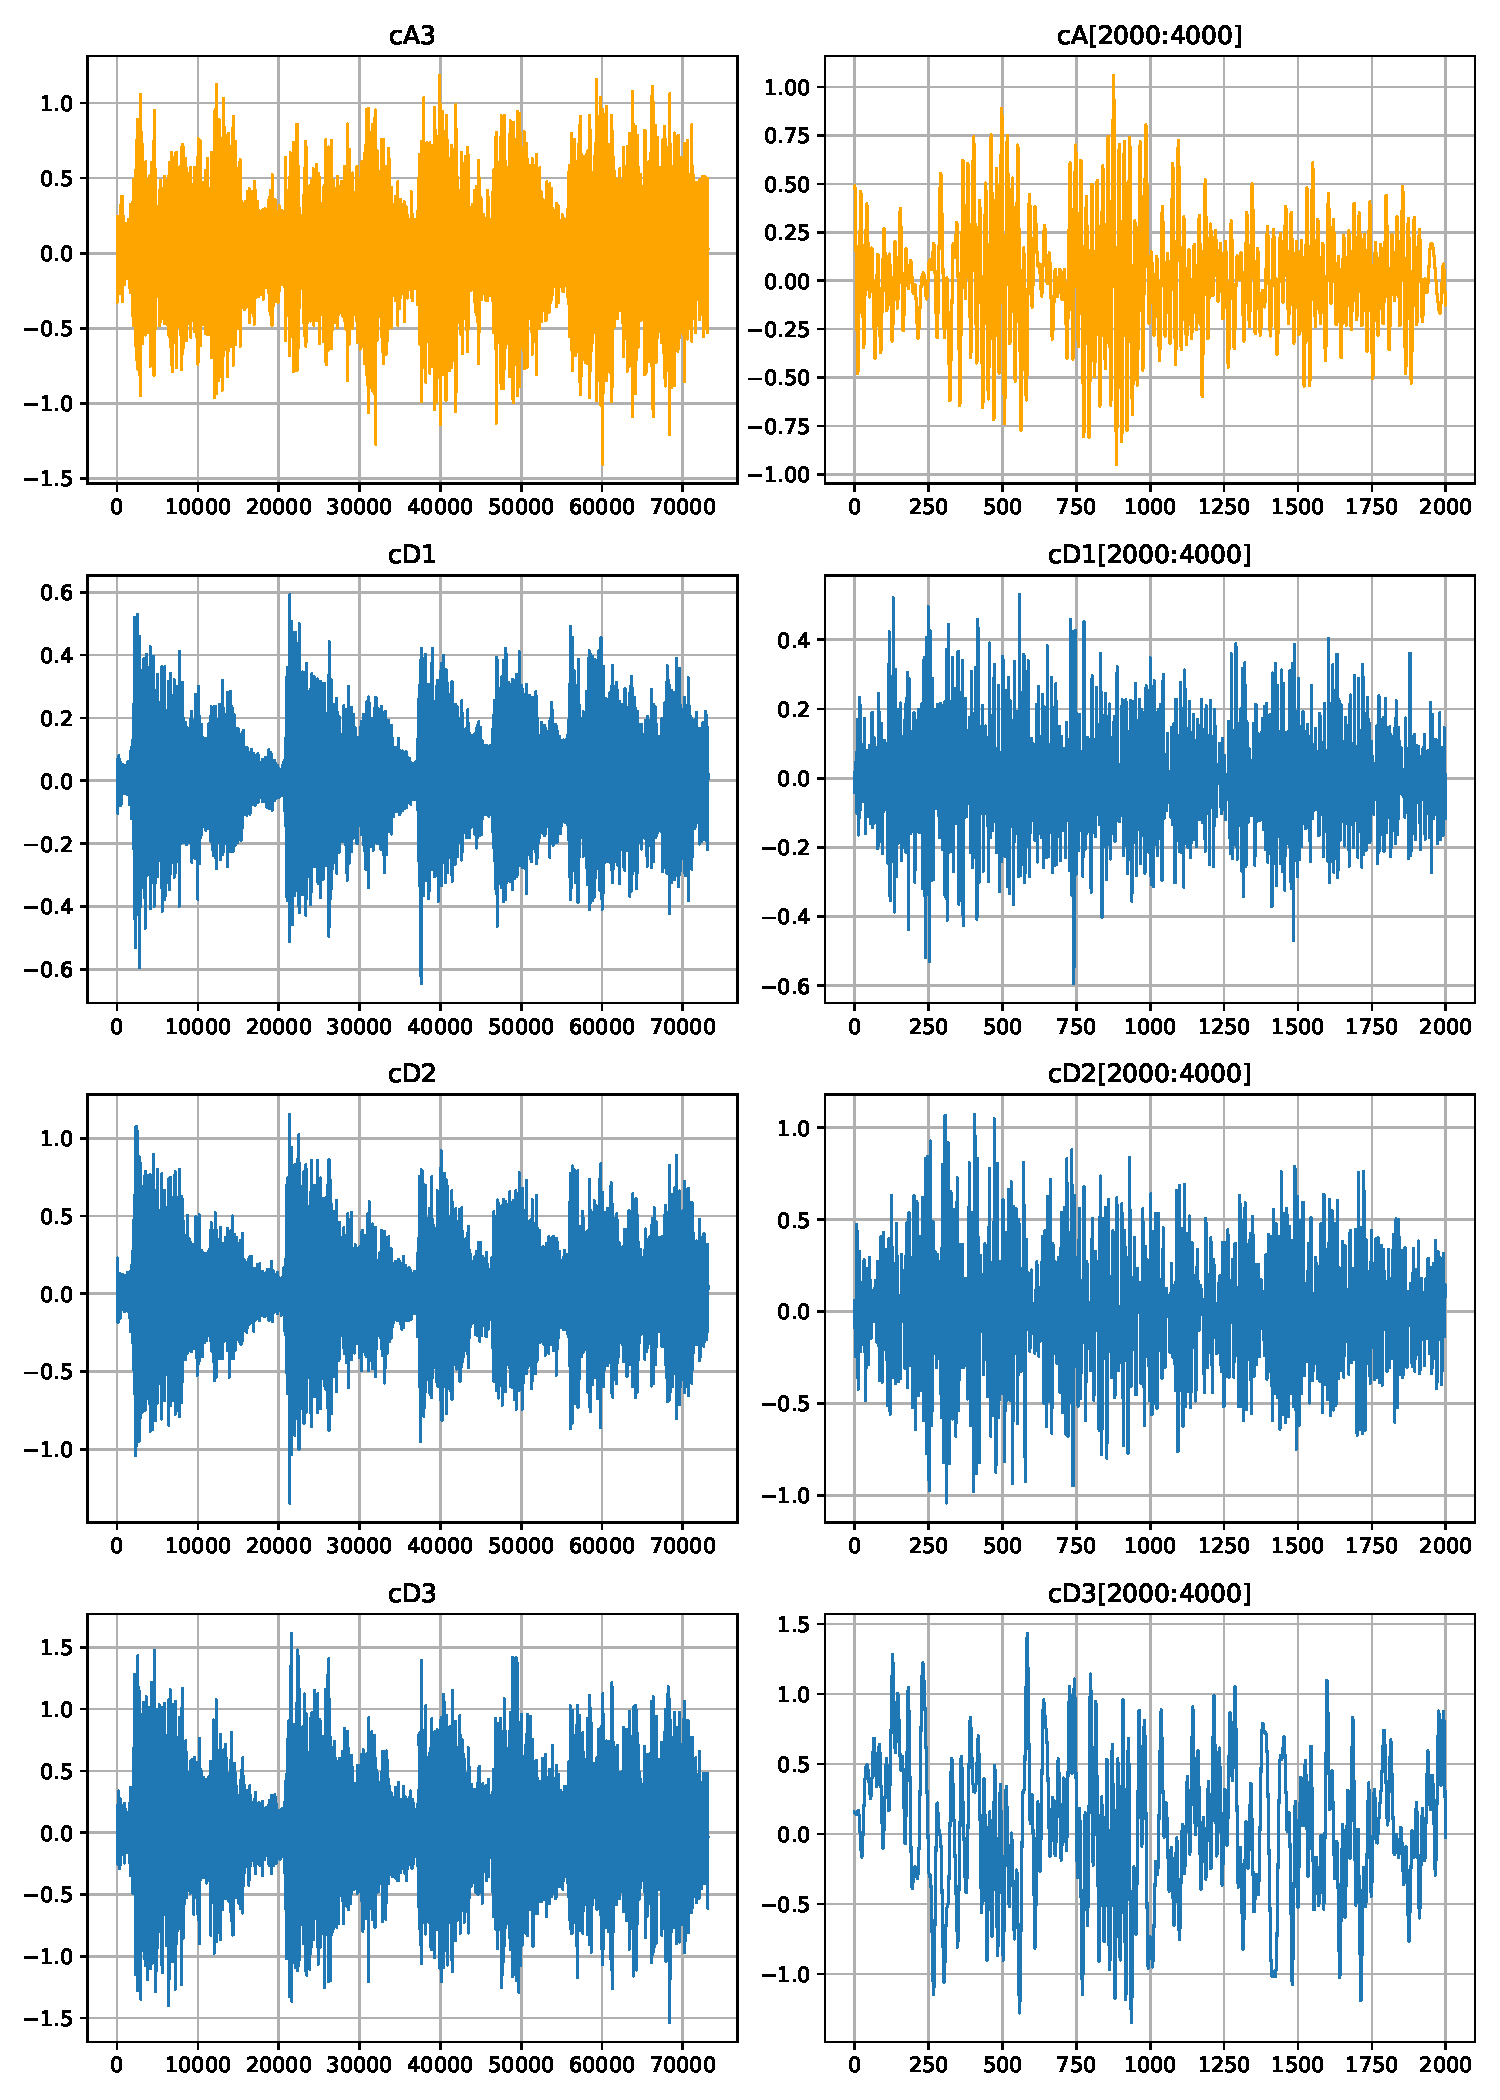
\includegraphics[width=1.1\textwidth]{./img/problem1-1-approximated-and-detailed-coeffs.pdf}}

    \caption{Approximated and detailed coefficients using DWT with \textit{db1} wavelet \textbf{3} levels deep. }
    \label{fig:problem1a}
\end{figure}

Figure \ref{fig:problem1a} shows the approximated and detailed coefficients computed using the \texttt{DWT} 3 levels deep using the \texttt{db1} wavelet. Both the approximate and the detailed coefficients have been resampled to have the same number of samples as the input signal in \texttt{Q1.mat}. This is done, to have a better visual representation of the coefficients. The first subplot at the top of the figure with the orange plot, are the approximated coefficients. Looking at the zoomed in interval, we can see that the coefficients are at a lower frequency that the input signal. This matches the theory, where the approximated coefficients are the frequency content at a lower frequency subband. The second, third and fourth subplots are the detailed coefficients at different transform levels. As the \texttt{DWT} is applied at the further levels the detail coefficients will be at a lower frequency compared to previous levels. This is also visible in the figure, where the detail coefficients at level 3 are at a lower frequency than the detail coefficients at level 2 etc.

% -- PROBLEM 1.B --------------------------------------------------------------

\begin{tcolorbox}[colback=red!5!white,colframe=red!75!black,title=Problem 1.b]
    Plot the reconstructed signal obtained using \verb|db1| and \verb|db2|.
\end{tcolorbox}

Using db1 should give a very similar signal to the original signal, while using db2 should give different signal, where the difference is noticeable.


\begin{figure}[H]
    \centering
    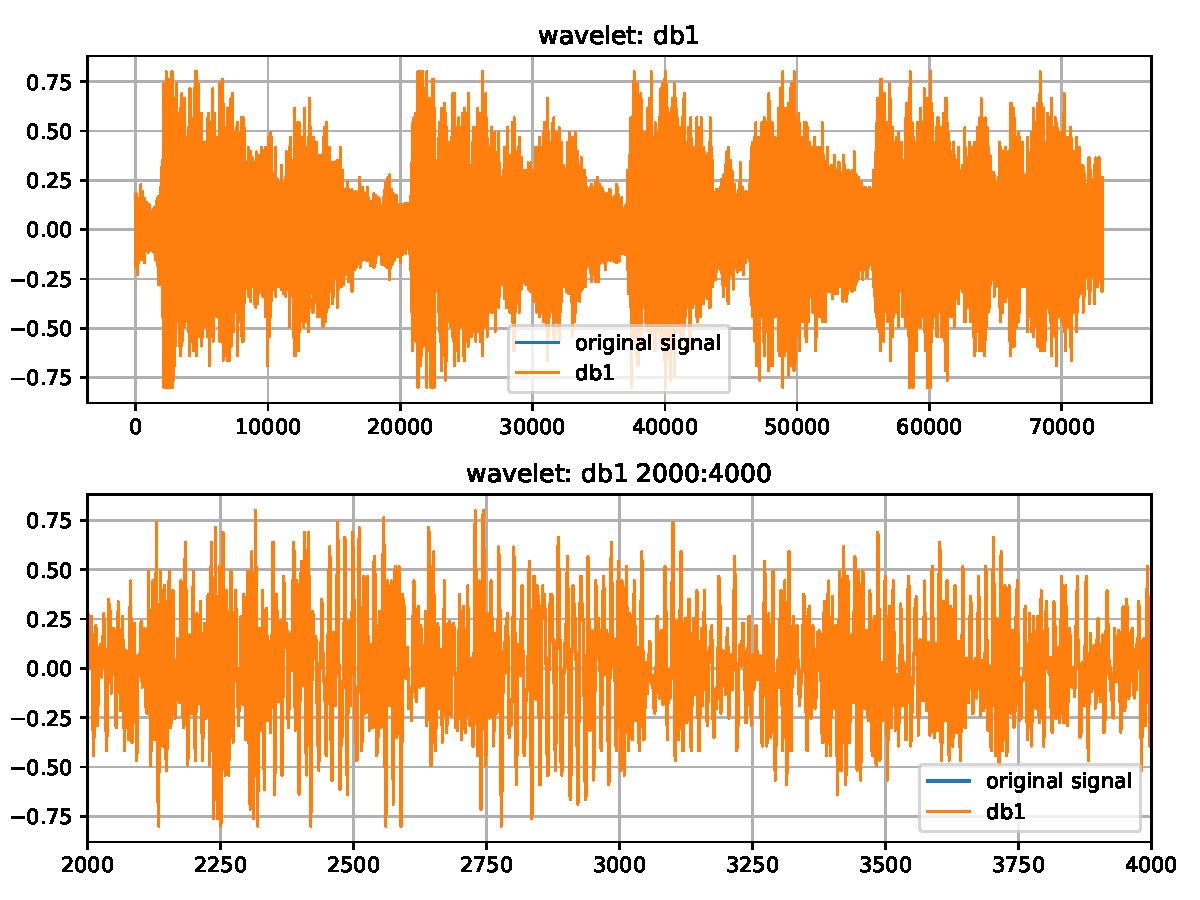
\includegraphics[width=\textwidth]{./img/problem1-2-reconstructed-signal-db1.pdf}
    \caption{Reconstructed signal using \textit{db1} wavelets.}
    \label{fig:y_reconstructed_with_db1}
\end{figure}

\begin{figure}[H]
    \centering
    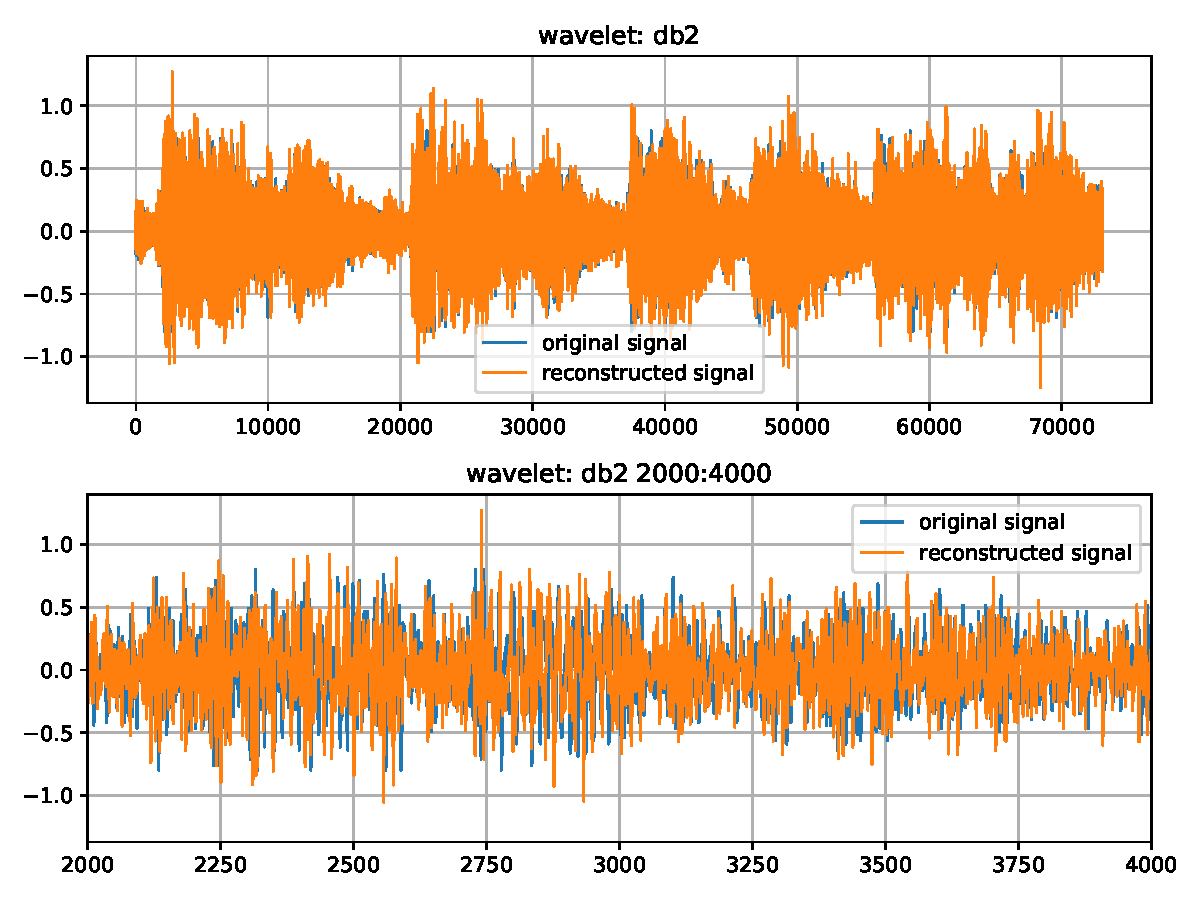
\includegraphics[width=\textwidth]{./img/problem1-2-reconstructed-signal-db2.pdf}
    \caption{Reconstructed signal using \textit{db2} wavelets.}
    \label{fig:y_reconstructed_with_db2}
\end{figure}


Figure \ref{fig:y_reconstructed_with_db1} and Figure \ref{fig:y_reconstructed_with_db2} shows the reconstructed signal using \textit{db1} and \textit{db2} wavelets respectively. The signal reconstructed using \textit{db1} wavelets is similar to the original signal, while the signal reconstructed using \textit{db2} wavelets is different. The difference is noticeable, especially, when zooming in on the signal, as can be seen in the third subplot of Figure \ref{fig:y_reconstructed_with_db2}, where the reconstructed signal does not overlap with the original signal. Instead the reconstructed appears to contain more higher frequency components. 

% -- PROBLEM 1.C --------------------------------------------------------------

\begin{tcolorbox}[colback=red!5!white,colframe=red!75!black,title=Problem 1.c]
    Hear (use \verb|sound| in MATLAB) the reconstructed signals using both wavelets.
    Report your observations.
\end{tcolorbox}

No audible difference can be heard between the \texttt{db1} reconstructed signal, and the original one. The vocals are clear, and no distortions are noticeable.

Listening to the audio of the reconstructed signal using \texttt{db2} wavelet, the vocals are still discernable, but the audio is distorted. The distortion is noticeable, and the audio is not as clear as the \texttt{db1} reconstructed signal.

% -- PROBLEM 1.D --------------------------------------------------------------

\begin{tcolorbox}[colback=red!5!white,colframe=red!75!black,title=Problem 1.d]
    Also, comment on the error obtained on the reconstructed signals for \verb|db1| and \verb|db2|.
\end{tcolorbox}

The error is calculated as the root mean squared error \textit{RMSE} between the original signal and the reconstructed signal, using the following formula:

\begin{equation}
    \text{RMSE}(x,y) = \sqrt{\frac{1}{N}\sum_{i=1}^{N}(x_i - y_{i})^2}
\end{equation}

\begin{table}[H]
    \label{tbl:reconstruction_error_with_db1_and_db2}
    \centering

    \begin{tabular}{c|c}
        \hline
        wavelet & RMSE \\
        \hline
        \texttt{db1} & $2.721 \cdot 10^{-19} \approx 0 $ \\
        \texttt{db2} & $1.001 \cdot 10^{-03}$ \\
    \end{tabular}

    \caption{Reconstruction error using \texttt{db1} and \texttt{db2} wavelets.}
\end{table}


The reconstruction error using \texttt{db1} wavelets is $2.721 \cdot 10^{-19} \approx 0$, while the reconstruction error using \texttt{db2} wavelets is $1.001 \cdot 10^{-03}$. The reconstruction error using \texttt{db1} wavelets is very small, and can be considered zero, with the minute difference from zero being due to the finite floating point representation. The reconstruction error using \texttt{db2} wavelets is much larger, and is noticeable when listening to the audio.

\ruler

\section*{Problem 2} \label{sec:problem2}

% problem introduction
\begin{tcolorbox}[colback=green!5!white,boxrule=0pt,frame empty]
    Add Gaussian noise ($\mu = 0$, $\sigma = 3$) to the original test
    EEG signal (\verb|Q2.mat|).
    Visualize both images (the original and its noisy version) side by side.
\end{tcolorbox}


\begin{figure}[H]
    \centering
    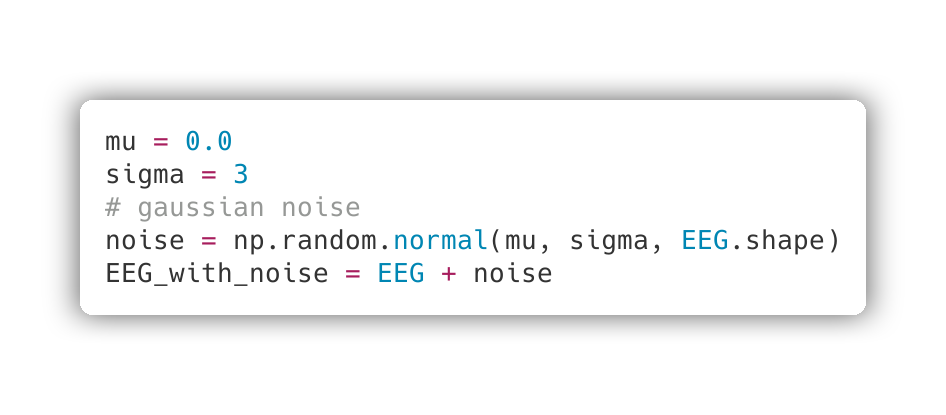
\includegraphics[width=0.8\textwidth]{./img/code_snippets/applying_noise_to_signal.png}
    \caption{Python code snippet for adding noise to a signal.}
    \label{code_snippet:applying_noise_to_signal}
\end{figure}

\begin{figure}[H]
    \centering
    \makebox[\textwidth][c]{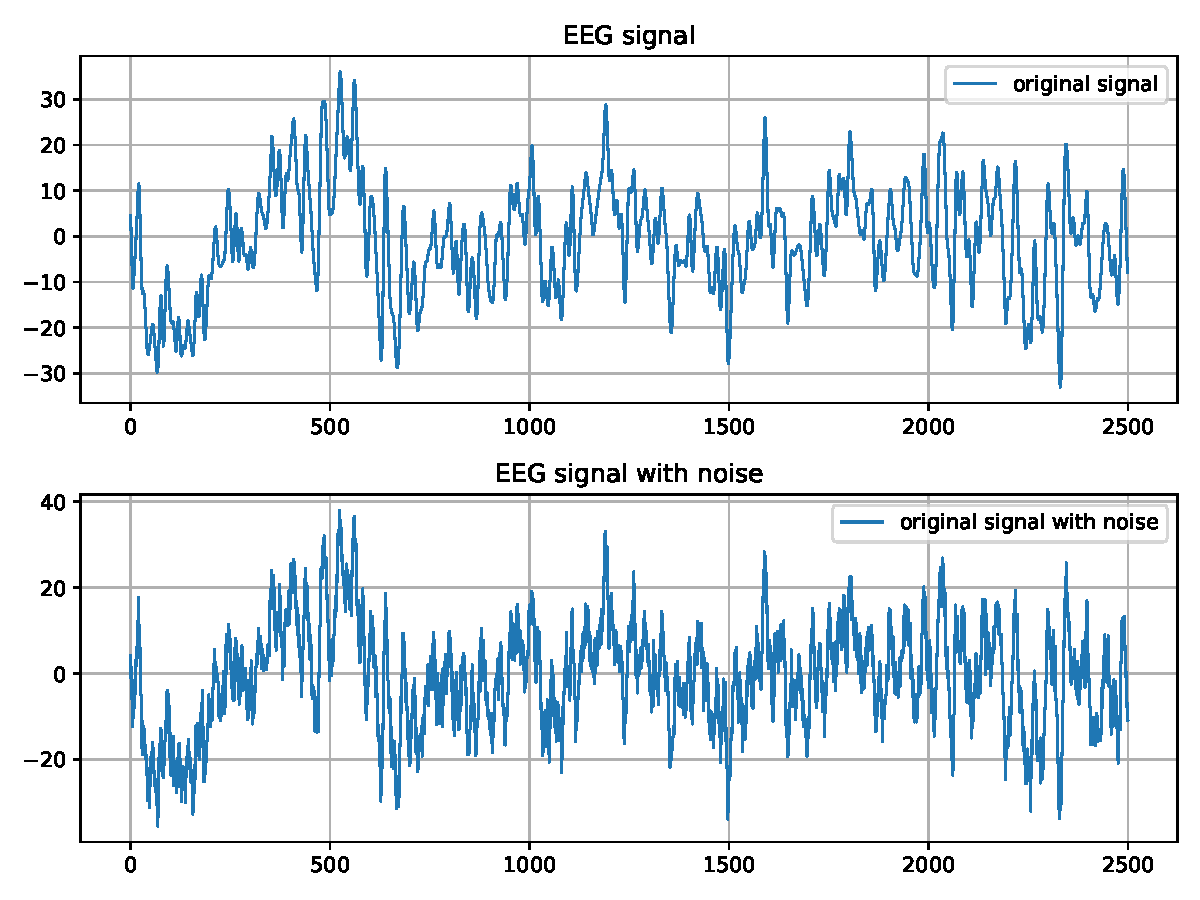
\includegraphics[width=1.0\textwidth]{./img/problem2-1-EEG-signal-with-and-without-noise.pdf}}
    \caption{The original EEG signal and its noisy version, where Gaussian noise with $\mu = 0$ and $\sigma = 3$ is added.}
    \label{fig:EEG_with_and_without_noise}
\end{figure}

\vspace{0.5cm}


% -- PROBLEM 2.A --------------------------------------------------------------

\begin{tcolorbox}[colback=green!5!white,colframe=green!75!black,title=Problem 2.a]
    Compute signal to noise ratio (SNR).
\end{tcolorbox}


\begin{equation}
    \text{SNR} = 10 \log_{10} \left( \frac{\text{signal power}}{\text{noise power}} \right) = 12.17 \text{ dB}
\end{equation}


% -- PROBLEM 2.B --------------------------------------------------------------

\begin{tcolorbox}[colback=green!5!white,colframe=green!75!black,title=Problem 2.b]
    Decompose the signal using wavedec (Haar, and db2).
\end{tcolorbox}

% -- PROBLEM 2.C --------------------------------------------------------------

\begin{tcolorbox}[colback=green!5!white,colframe=green!75!black,title=Problem 2.c]
    Plot the subbands obtained using Haar and db2 decomposition.
\end{tcolorbox}

\begin{figure}[H]
    \centering
    \makebox[\textwidth][c]{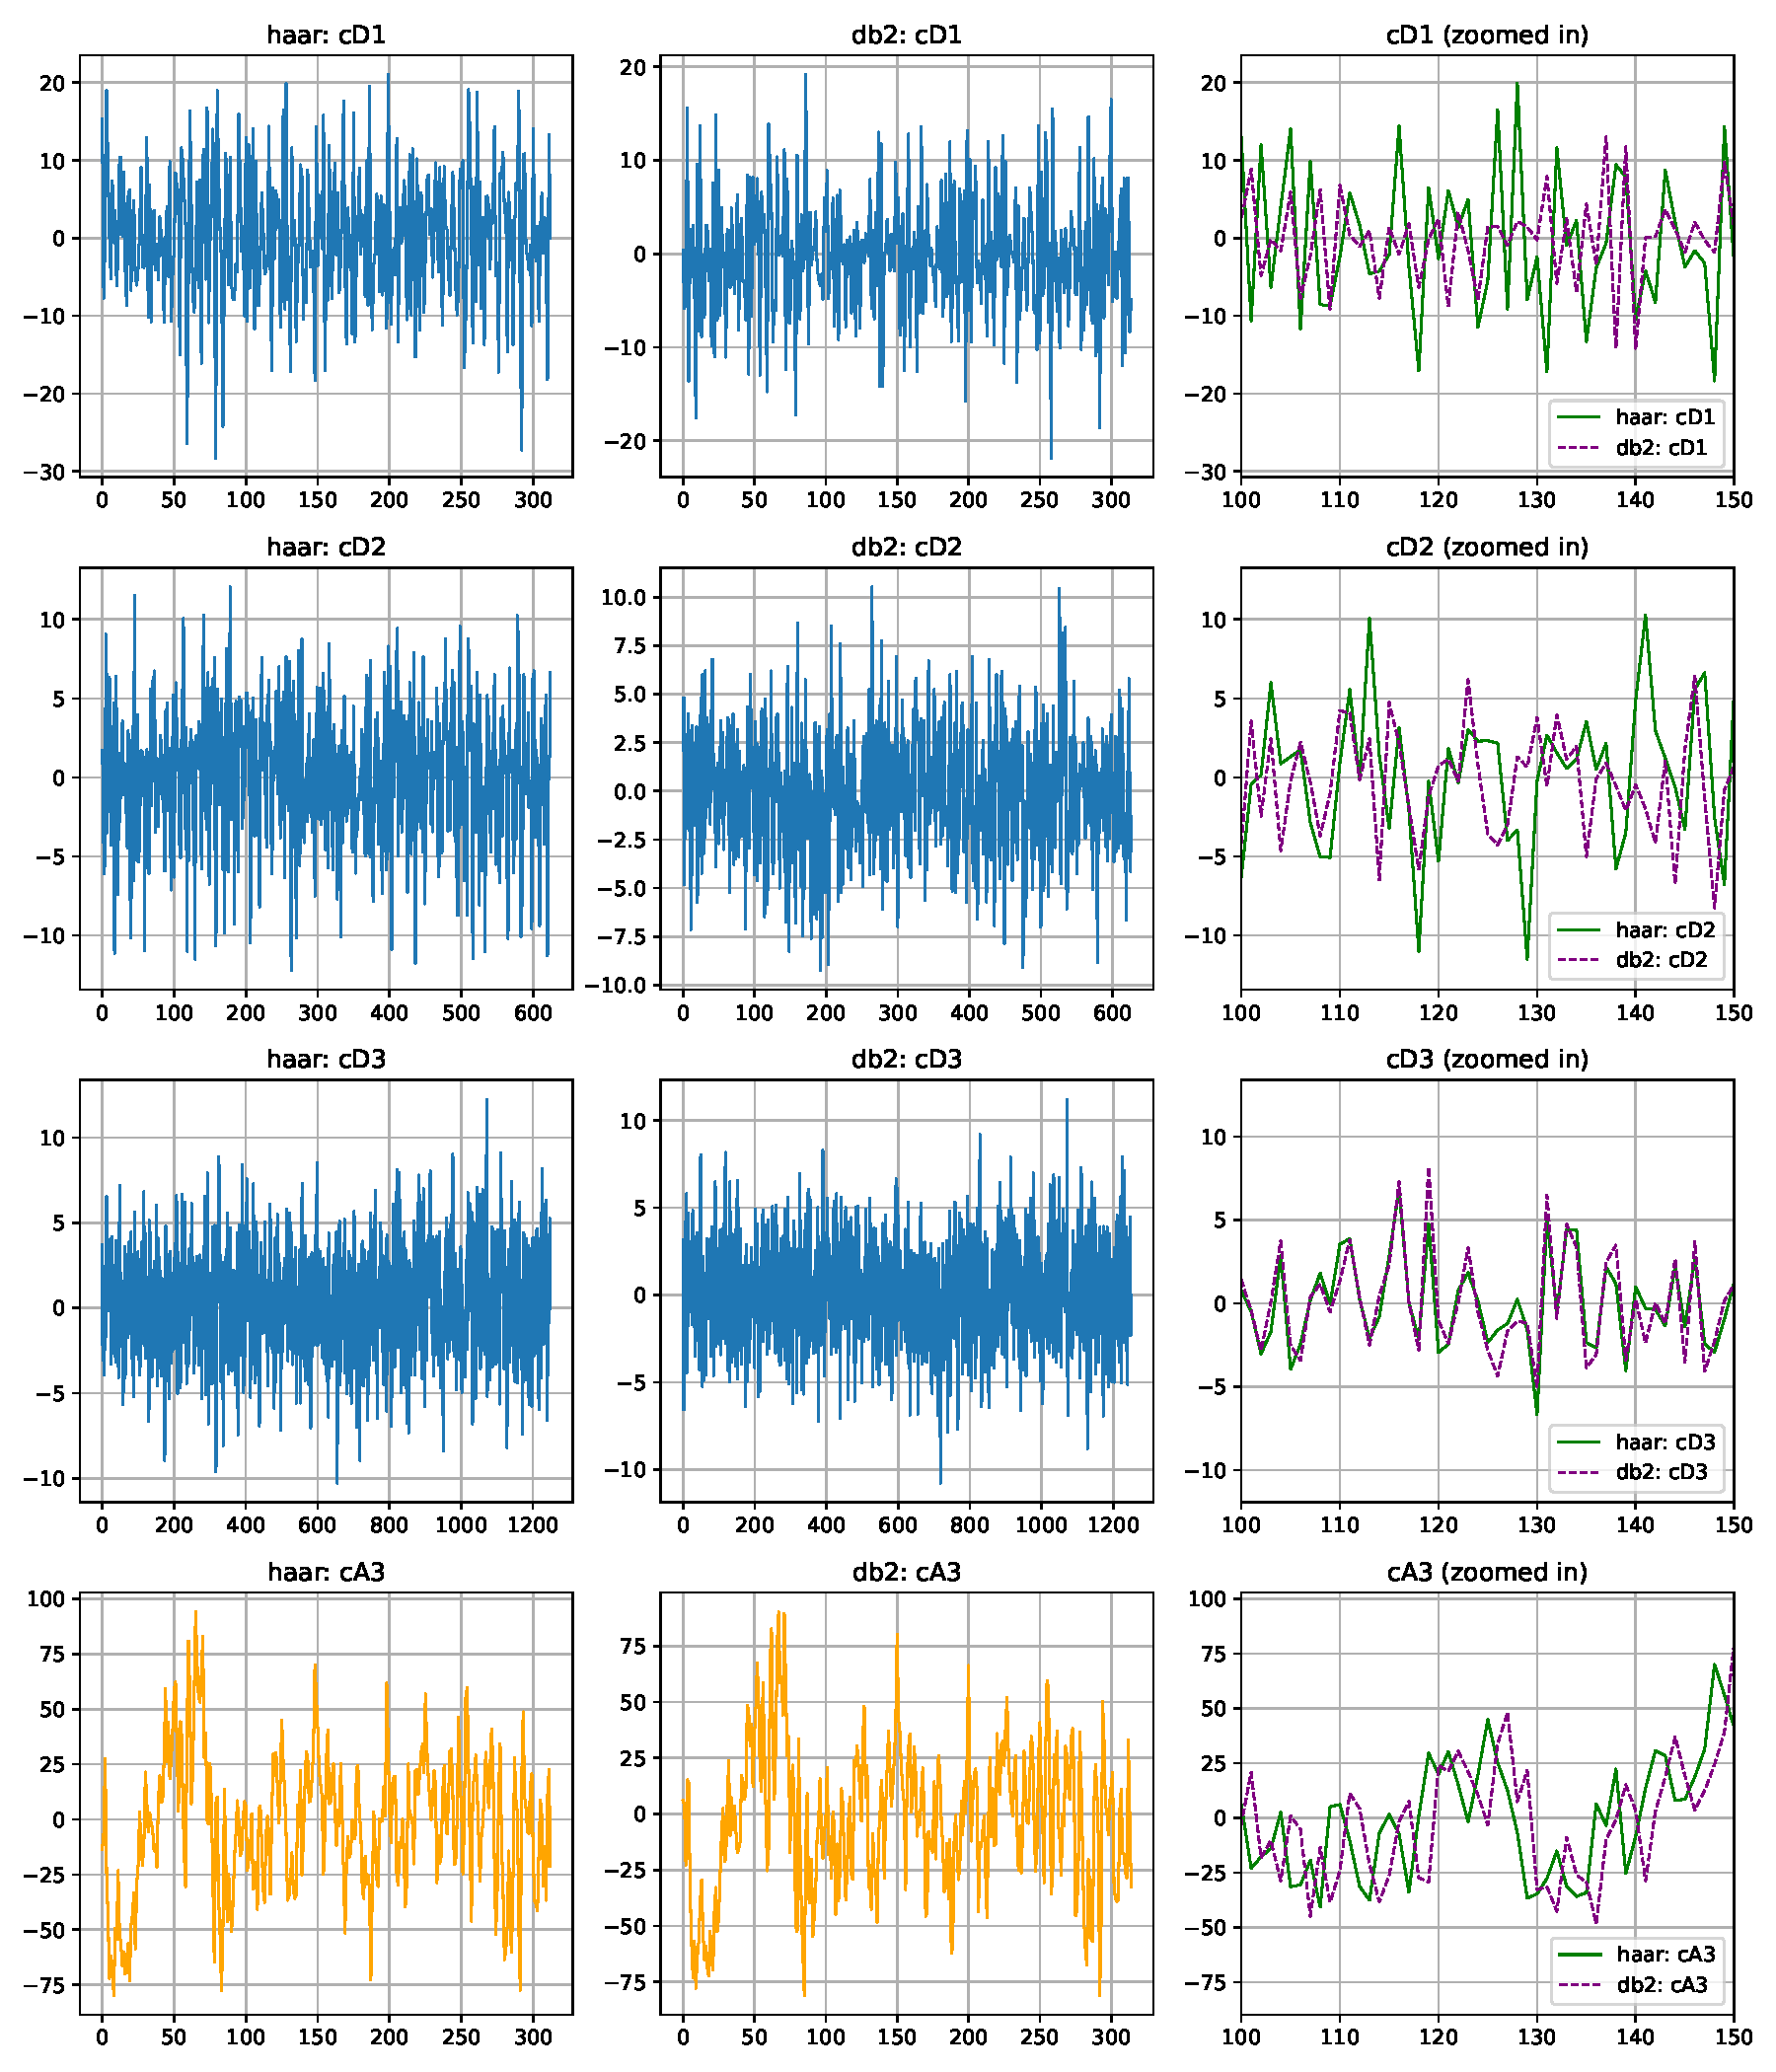
\includegraphics[width=1.1\textwidth]{./img/problem2c_haar_and_db2_subband_decomposition.pdf}}
    \caption{Subbands of the EEG signal using \texttt{haar} and \texttt{db2} wavelets.}
    \label{fig:problem2c_haar_and_db2_subband_decomposition}
\end{figure}

% -- PROBLEM 2.D --------------------------------------------------------------

\begin{tcolorbox}[colback=green!5!white,colframe=green!75!black,title=Problem 2.d]
    Observe the subbands and list your observations.
\end{tcolorbox}

Figure \ref{fig:problem2c_haar_and_db2_subband_decomposition} shows the subbands of the EEG signal using \texttt{haar} and \texttt{db2} wavelets. Looking at all of the coefficients, both approximate and detail, for both wavelets i.e. column 1 and 2 in \ref{fig:problem2c_haar_and_db2_subband_decomposition} it is very diffecult to see any difference between the two wavelets. The coefficients are very similar, and the difference is not immediately noticeable. The third column shows the coefficients of both wavelets zoomed in on the sample interval $[100, 150]$. In this view the difference between the two wavelets are more apparent. For \texttt{cD1} and \texttt{cD2} there is a difference between the captured frequency. In \texttt{cD3} the detail coefficients are almost identical, and for \texttt{cA3} the approximate coefficients are almost identical, only differing in the phase.



\ruler


\section*{Problem 3} \label{sec:problem3}

% problem introduction
\begin{tcolorbox}[colback=blue!5!white,boxrule=0pt,frame empty]
    Perform DWT on the given EEG signal (\verb|Q3.mat|) and threshold the detail coefficients
    the following way:
    \vspace{0.5em}
    \begin{itemize}
        \item Select a threshold $T = \sigma \sqrt{2 \log(n)}$ where n is the number of detail coefficients 
        and $\sigma$ is an estimate of the noise level.
        \item Set all detail coefficients smaller than $T$ to zero.
    \end{itemize}
\end{tcolorbox}


\vspace{0.5cm}

A good estimate of the noise level is the standard deviation of the noise. This can be calculated using the following equation
\footnote{This equation for the estimation of the noise level is taken from the \textit{WaveletDenoising.m} file, presented in week 12 of the course.}:

\begin{equation}
    \hat{\sigma} = \frac{\mathrm{median}(|cD|)}{0.6745} = 1.997
\end{equation}

Where $cD$ is the detail coefficients of the DWT. The median is used to reduce the effect of outliers.

The tested values for $\sigma$ are:

\begin{equation}
    \mathbf{\sigma} = [ \hat{\sigma}, 0.5, 1, 2, 4 ]
\end{equation}

\begin{figure}[H]
    \centering
    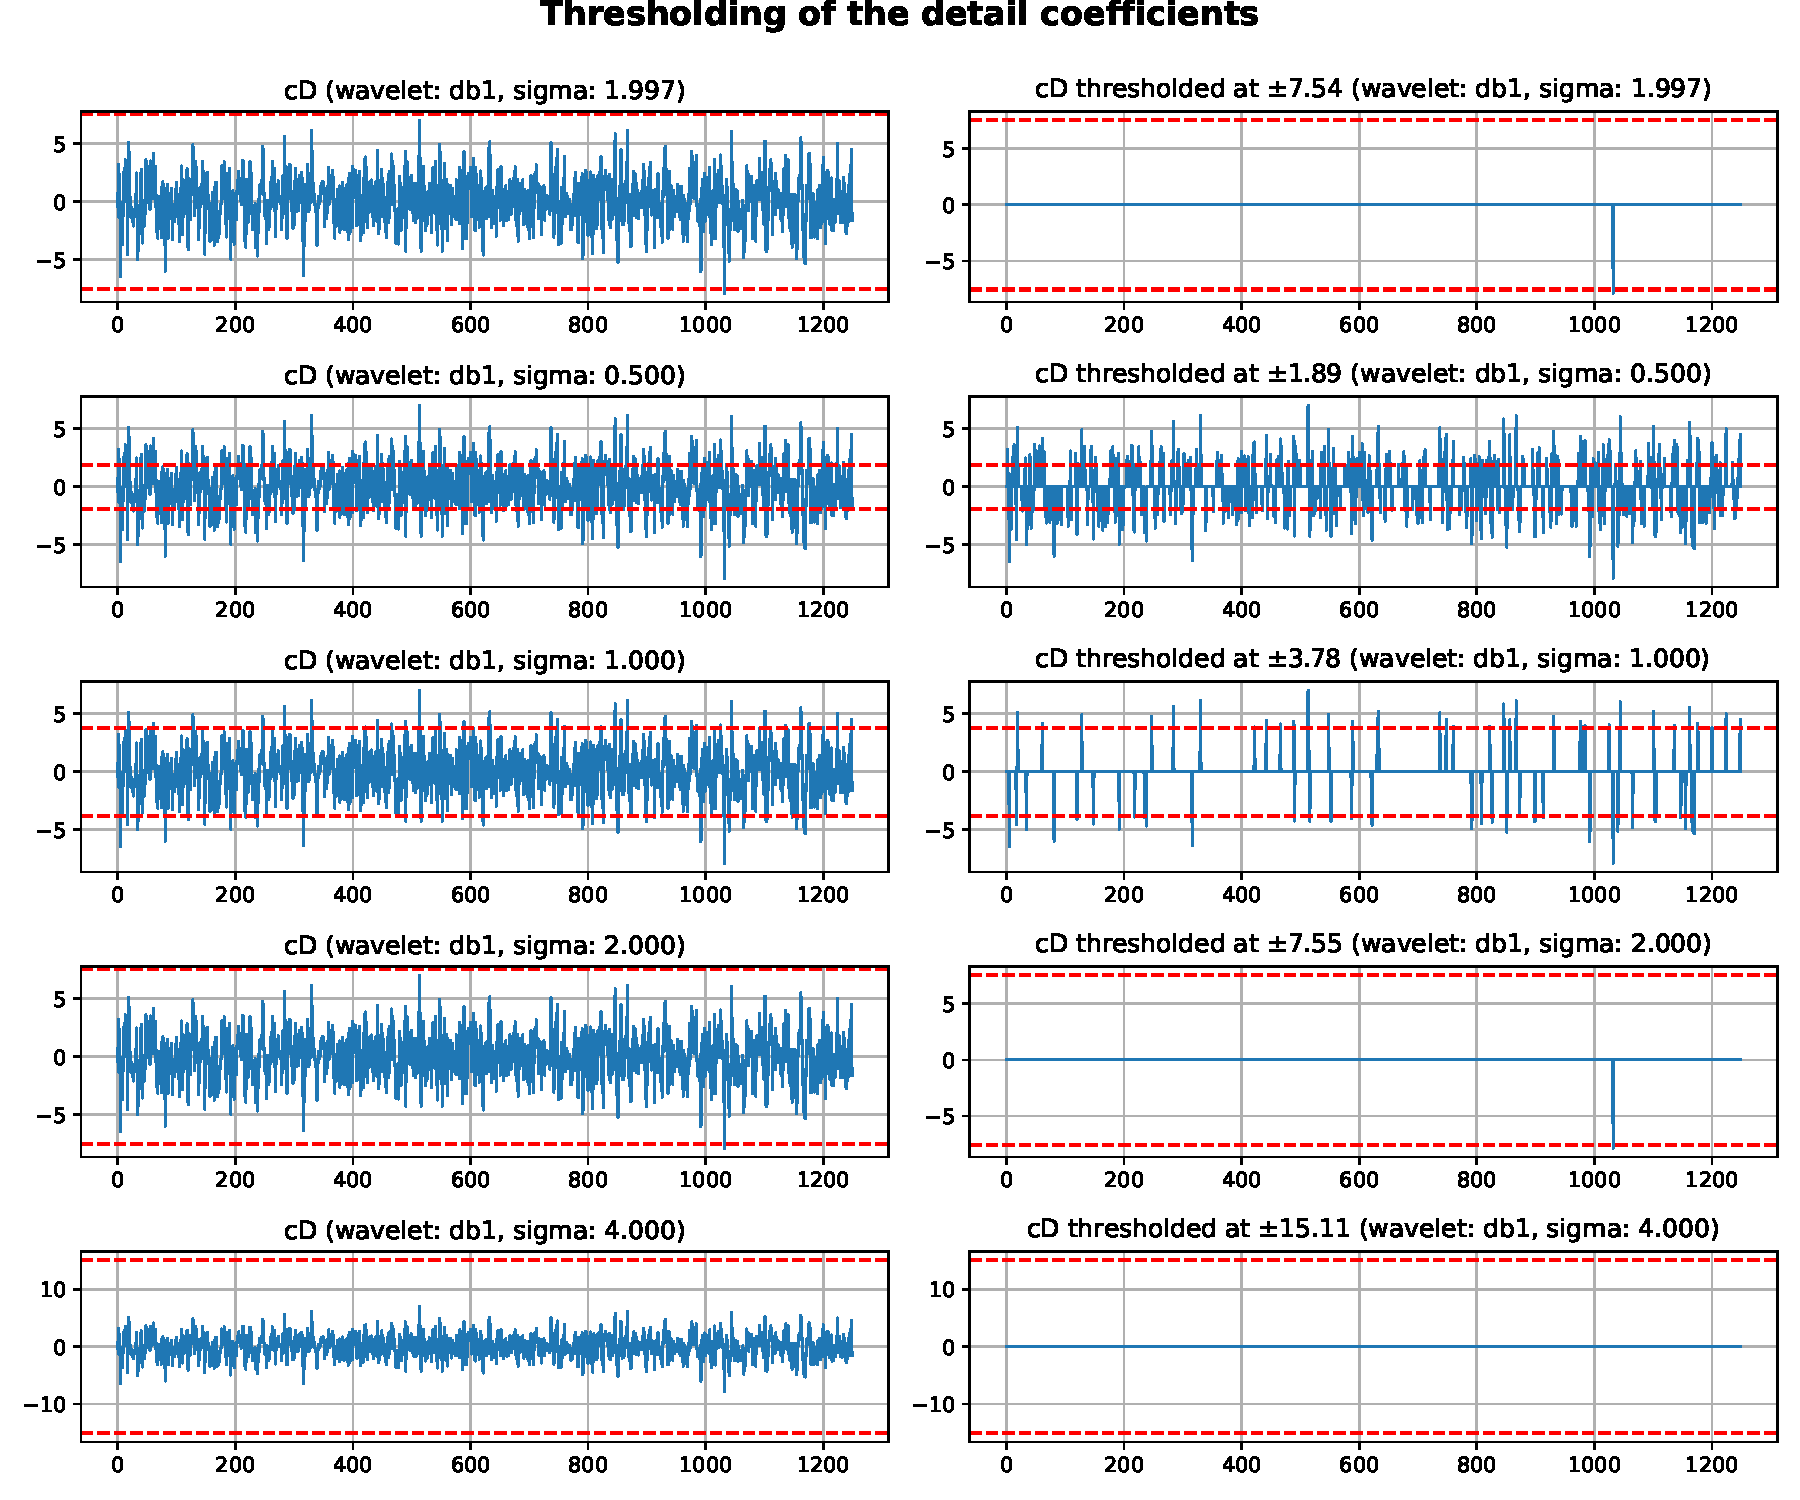
\includegraphics[width=\textwidth]{./img/problem3-thresholding-of-detail-coefficients.pdf}
    \caption{The left column shows the detail coefficients of the noisy EEG signal. The detail coefficients are computed using the Discrete Wavelet Transform with the \textrm{db1} wavelet at a level of 1. The right column shows the detail coefficients after thresholding with $T = \sigma \sqrt{2 \log(n)}$. The threshold is computed for different values of $\sigma$. The threshold is indicated by the dashed red line.}
    \label{fig:problem3thresholding}
\end{figure}

Figure \ref{fig:problem3thresholding} shows the detail coefficients of the \texttt{DWT} with the \texttt{db1} wavelet. Aswell as the thresholded detail coefficients for the different values of $\sigma$. At $\sigma\ >\ 2$, allmost all detail coefficients are set to zero. 


% -- PROBLEM 3.A --------------------------------------------------------------

\begin{tcolorbox}[colback=blue!5!white,colframe=blue!75!black,title=Problem 3.a]
    Compute the SNR for different $\sigma$ values and values of $\sigma = \left \lbrace 0.5, 1, 2, 4 \right \rbrace$.
\end{tcolorbox}


\begin{table}[H]
    \label{tbl:snr_values_for_different_sigmas}
    \centering

    \begin{tabular}{c|c}
        \hline
        $\sigma$ & SNR \\
        \hline
        
        $\hat{\sigma}$ & 16.82 dB \\
        0.5 & 16.87 dB \\
        1.0 & 16.84 dB \\
        2.0 & 16.82 dB \\
        4.0 & 16.82 dB \\

    \end{tabular}

    \caption{The SNR for different values of $\sigma$.}
\end{table}


% -- PROBLEM 3.B --------------------------------------------------------------

\begin{tcolorbox}[colback=blue!5!white,colframe=blue!75!black,title=Problem 3.b]
    Plot the original, noisy, and denoised signal in anyone case.
\end{tcolorbox}


\begin{figure}[H]
    \label{fig:problem3b_plot1}
    \centering
    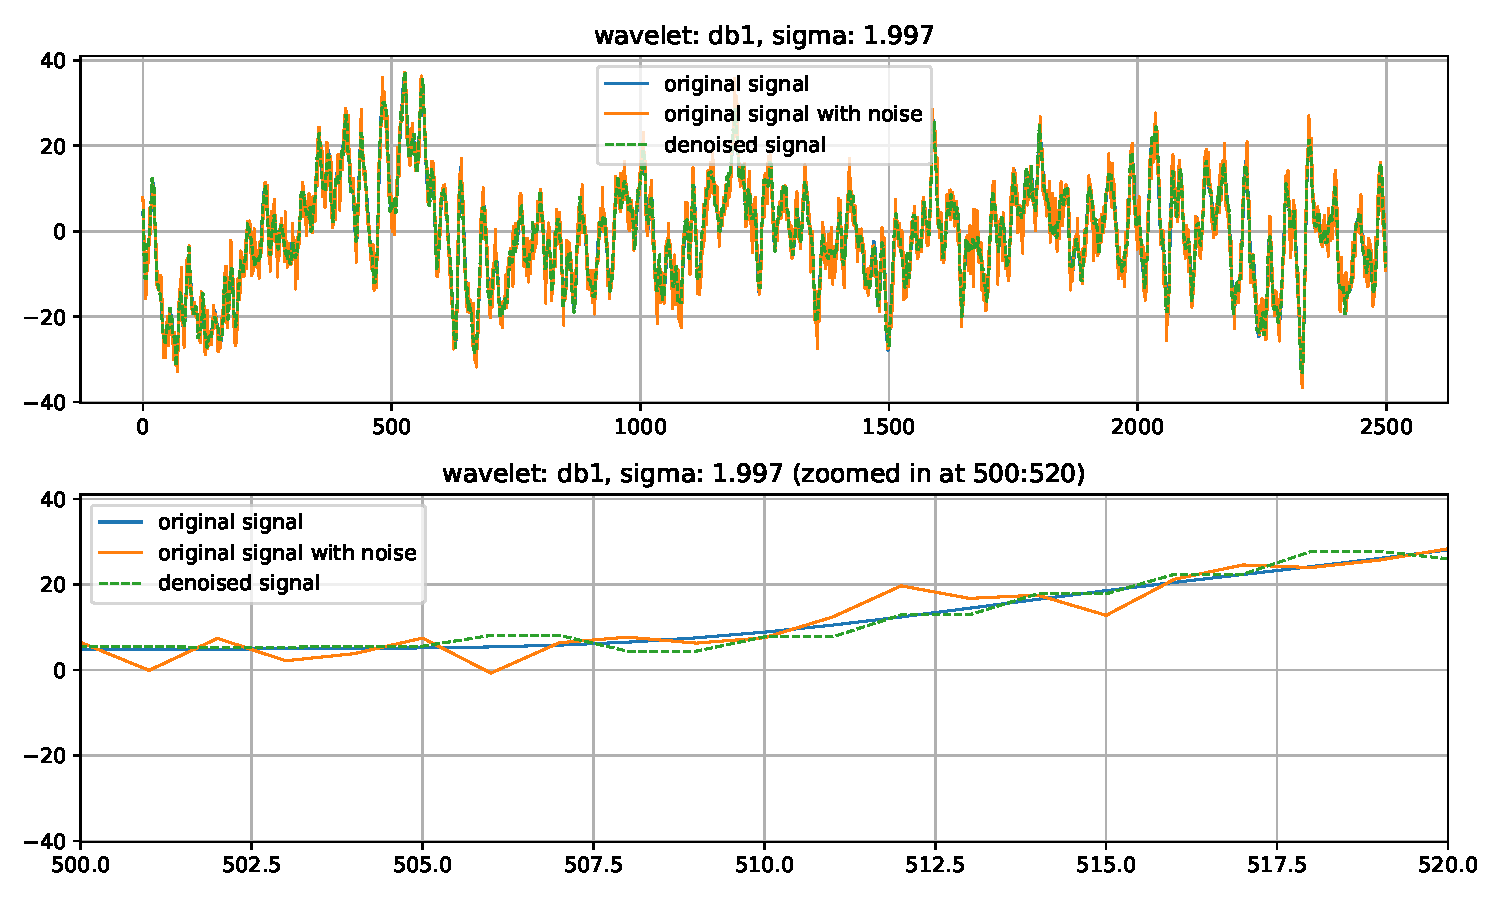
\includegraphics[width=0.9\textwidth]{./img/problem3-denoised-signal-wavelet-db1-sigma-1.997.pdf}
    \caption{The original EEG signal, the noisy EEG signal, and the denoised EEG signal. The denoising is done using the \texttt{db1} wavelet and $\sigma = \hat{\sigma}$.}
\end{figure}


\begin{figure}[H]
    \label{fig:problem3b_plot2}
    \centering
    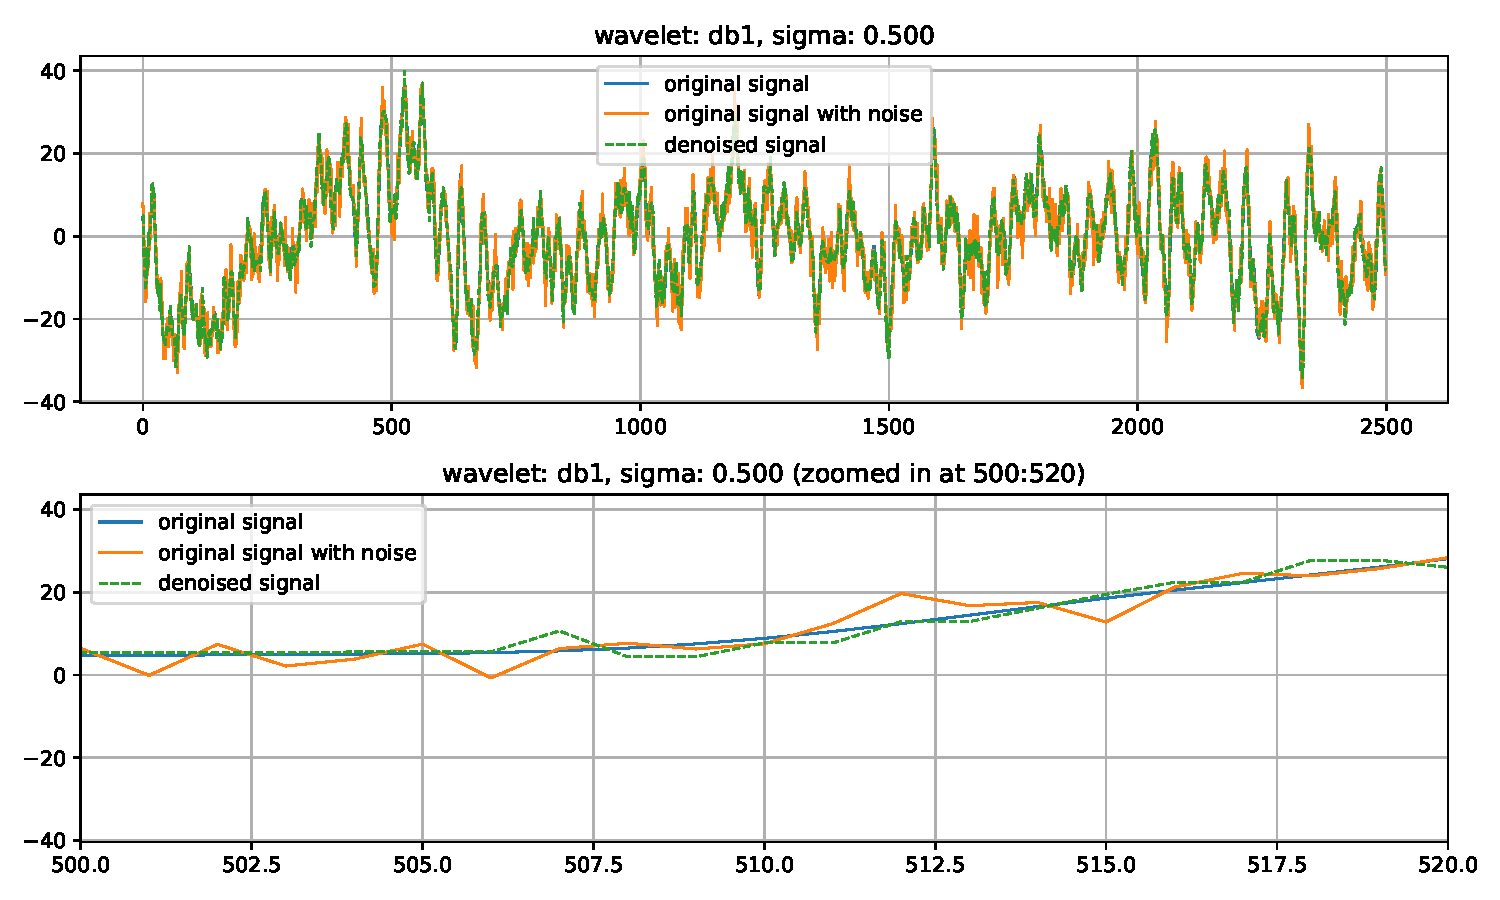
\includegraphics[width=0.9\textwidth]{./img/problem3-denoised-signal-wavelet-db1-sigma-0.500.pdf}
    \caption{The original EEG signal, the noisy EEG signal, and the denoised EEG signal. The denoising is done using the \texttt{db1} wavelet and $\sigma = 0.5$.}
\end{figure}


\begin{figure}[H]
    \label{fig:problem3b_plot3}
    \centering
    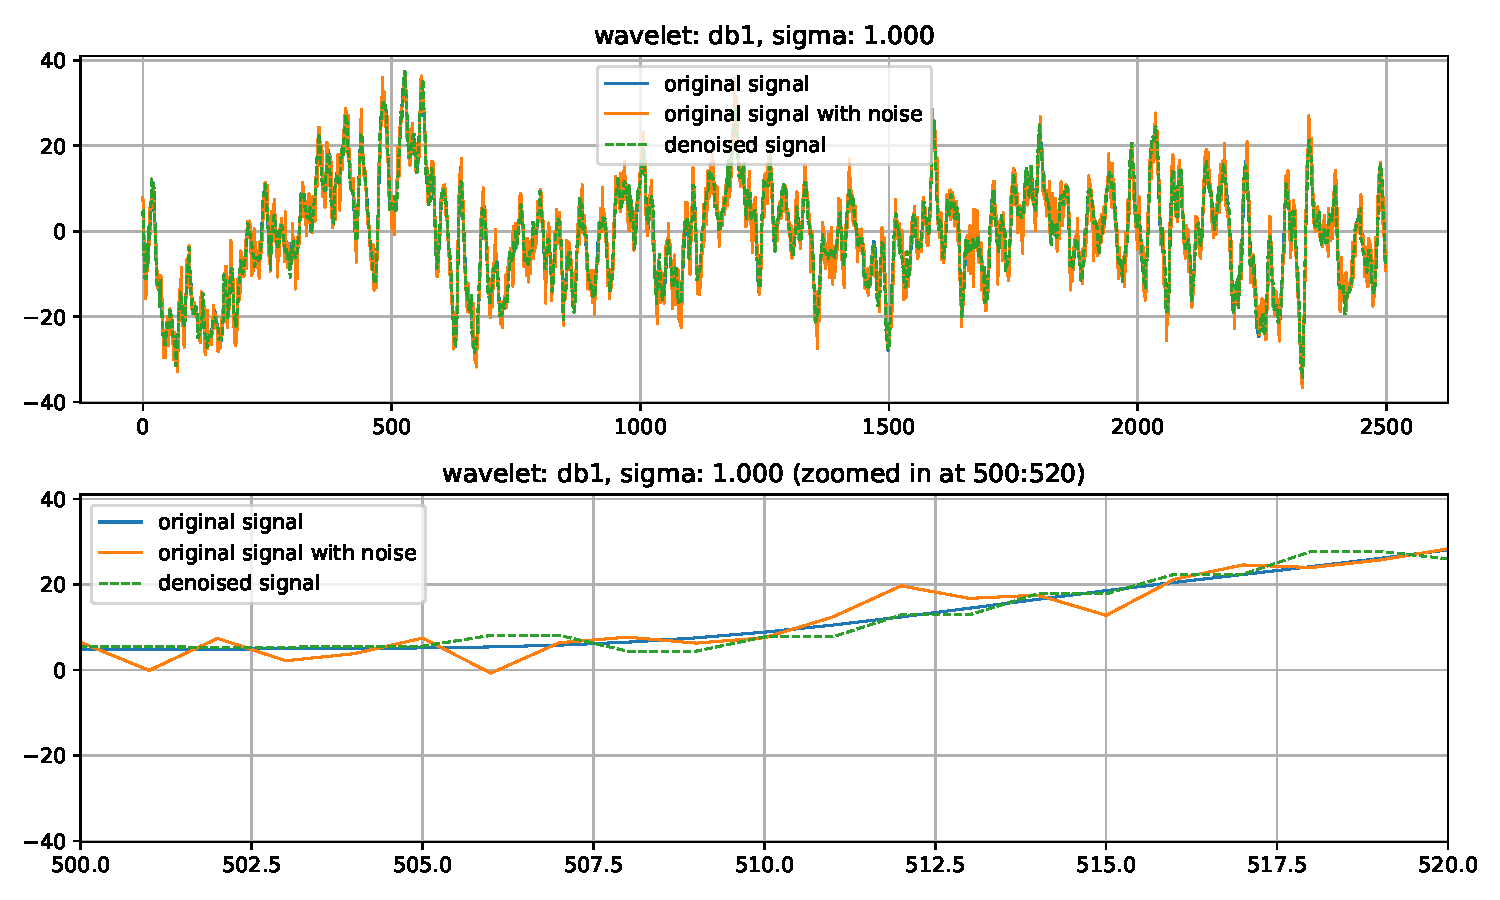
\includegraphics[width=0.9\textwidth]{./img/problem3-denoised-signal-wavelet-db1-sigma-1.000.pdf}
    \caption{The original EEG signal, the noisy EEG signal, and the denoised EEG signal. The denoising is done using the \texttt{db1} wavelet and $\sigma = 1$.}
\end{figure}

\begin{figure}[H]
    \label{fig:problem3b_plot4}
    \centering
    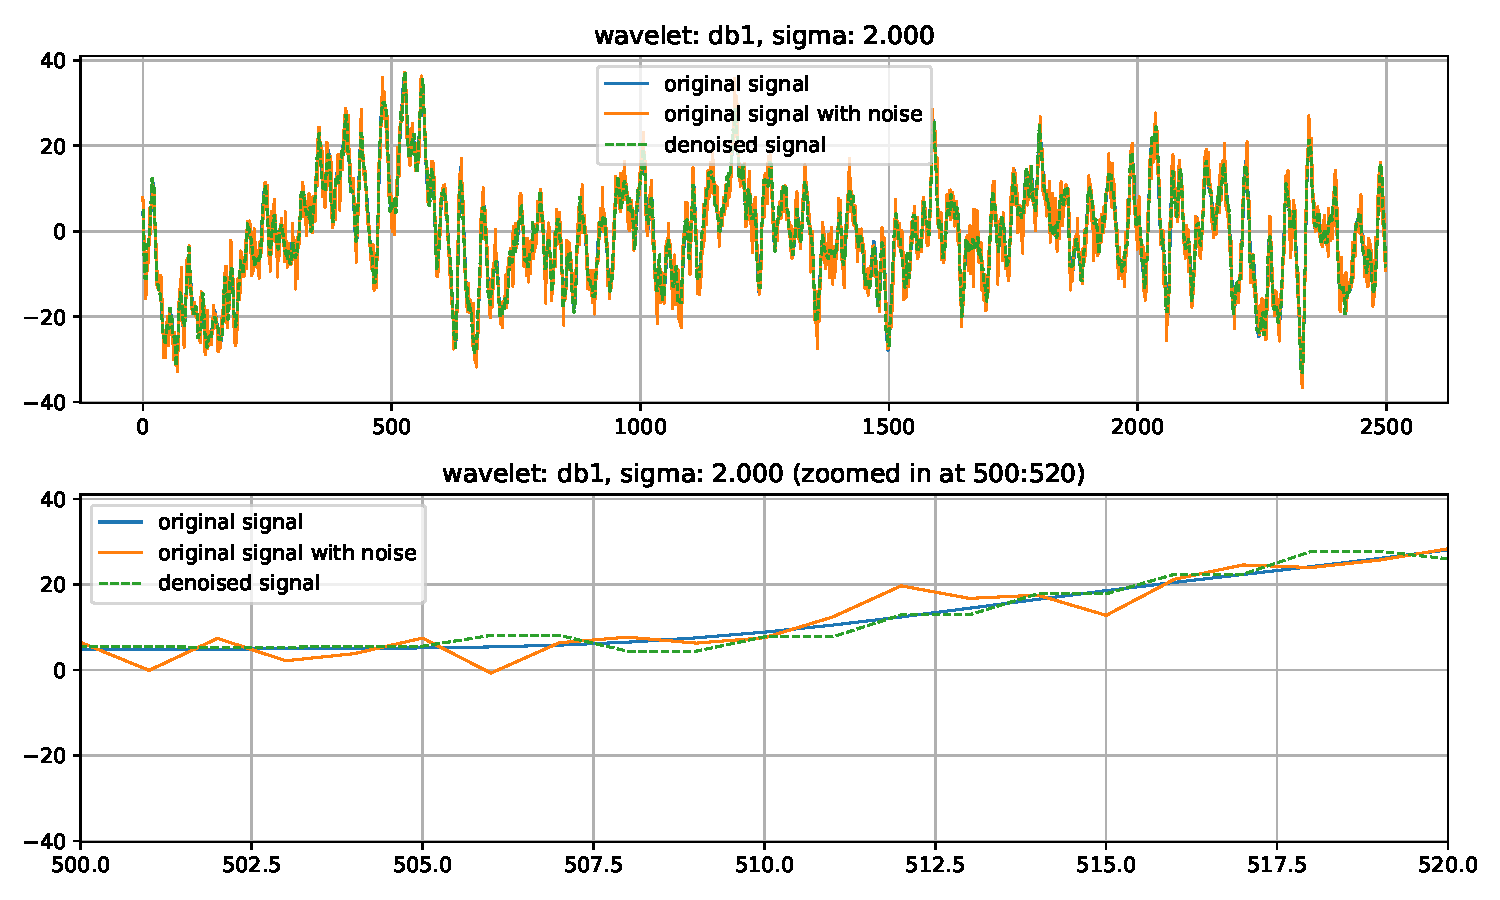
\includegraphics[width=0.9\textwidth]{./img/problem3-denoised-signal-wavelet-db1-sigma-2.000.pdf}
    \caption{The original EEG signal, the noisy EEG signal, and the denoised EEG signal. The denoising is done using the \texttt{db1} wavelet and $\sigma = 2$.}
\end{figure}

\begin{figure}[H]
    \label{fig:problem3b_plot5}
    \centering
    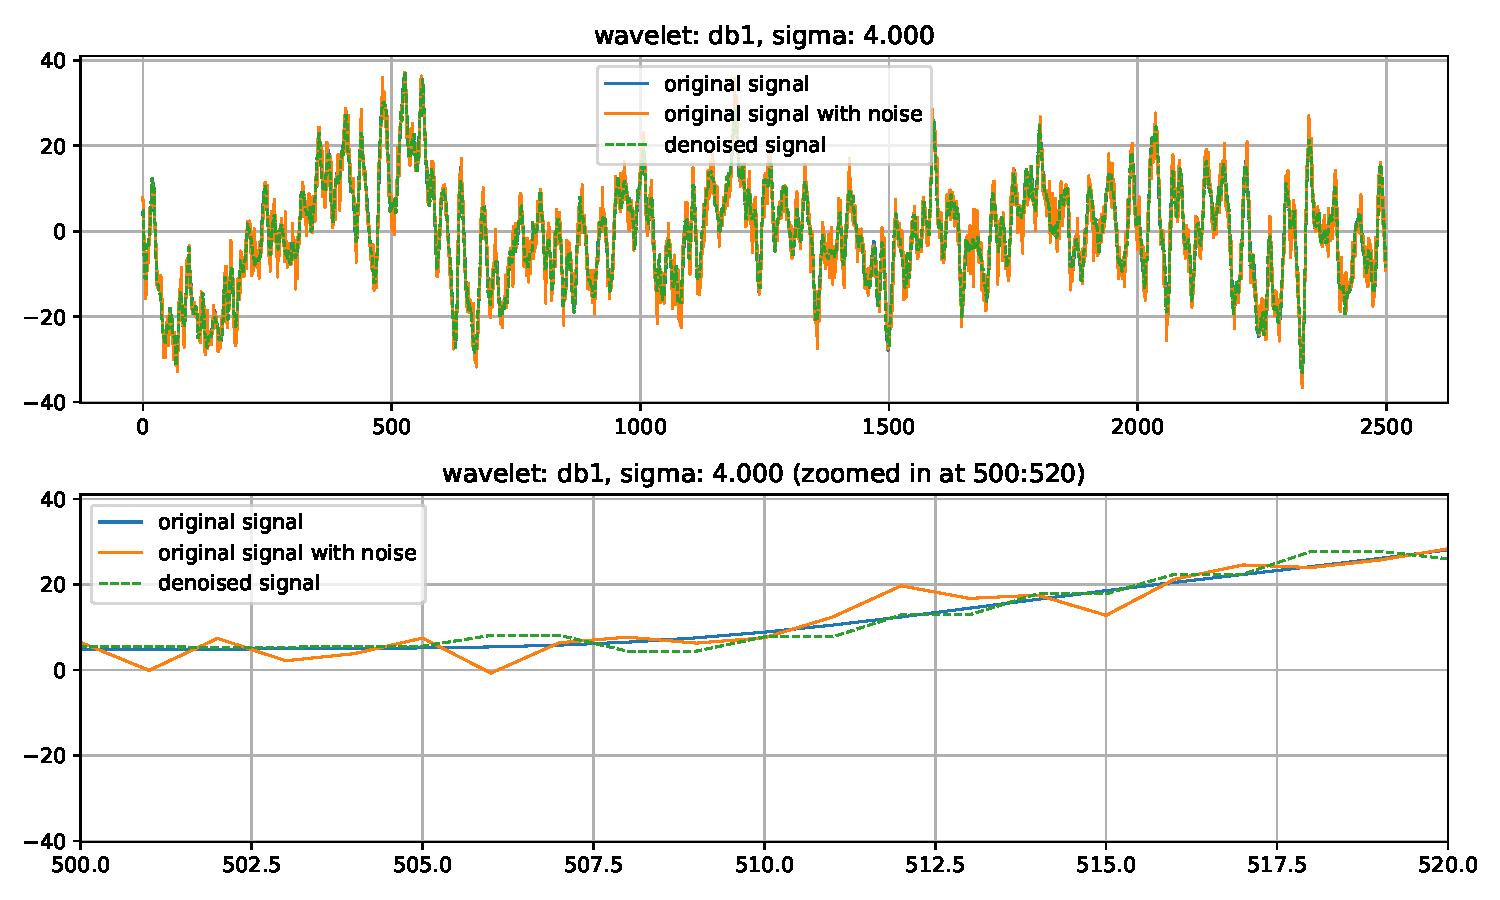
\includegraphics[width=0.9\textwidth]{./img/problem3-denoised-signal-wavelet-db1-sigma-4.000.pdf}
    \caption{The original EEG signal, the noisy EEG signal, and the denoised EEG signal. The denoising is done using the \texttt{db1} wavelet and $\sigma = 4$.}
\end{figure}




% -- PROBLEM 3.C --------------------------------------------------------------

\begin{tcolorbox}[colback=blue!5!white,colframe=blue!75!black,title=Problem 3.c]
    Evaluate the RMSE and comment on your interpretations for each case.
\end{tcolorbox}

\todo{finish}

\begin{table}[H]
    \label{tbl:rmse_values_for_different_sigmas}
    \centering

    \begin{tabular}{c|c}
        \hline
        $\sigma$ & RMSE \\
        \hline
        
        $\hat{\sigma}$ & 0.238 \\
        0.5 & 0.237 \\
        1.0 & 0.238 \\
        2.0 & 0.238 \\
        4.0 & 0.238 \\

    \end{tabular}

    \caption{The RMSE for different values of $\sigma$.}
\end{table}
